\documentclass[
reprint,
amsmath,amssymb,
aip,
jap,
floatfix,
]{revtex4-2}

\usepackage{graphicx}
\usepackage{dcolumn}
\usepackage{bm}
\usepackage{siunitx}
\usepackage{xcolor, soul}
%\usepackage[dvipsnames]{xcolor}
%\usepackage{soul}
%\usepackage[normalem]{ulem}


\begin{document} 

\preprint{APS/123-QED}

\title{An investigation of the coupling of phonon-polaritons with plasmon-polaritons in hBN/nanopatterned Au layered devices}

\author{J. D. T. Heneghan}
\email{dermoth@uga.edu}
\author{W. M. Dennis}
\email{drd@uga.edu}
\affiliation{
  Department of Physics and Astronomy,\\
  University of Georgia,\\
  Athens, GA 30602-2451, U.S.A.\\
}

\date{\today}

\chapter[An Investigation of the Polariton-Plasmon Coupling in hBN on Nanopatterned Ag Layered Structures]
  {An Investigation of the Polariton-Plasmon Coupling in hBN on Nanopatterned Ag Layered Structures%
  \footnote{D.J.T Heneghan, W. M. Dennis,2021, 
  \emph{Journal TBD}, Vol. TBD, No. TBD. \indent\indent Reprinted here with permission of publisher and authors.}}
  \label{chapter:Ag_hBN}

  \newpage


	Electromagnetic simulations were performed using the Finite-Difference Time-Domain (FDTD) method    using an in-house designed code. The FDTD method numerically integrates the Maxwell curl equations with second-order accuracy as detailed in Ref. \cite{Wan:16}.

      \begin{figure*}[!htb]
        \centering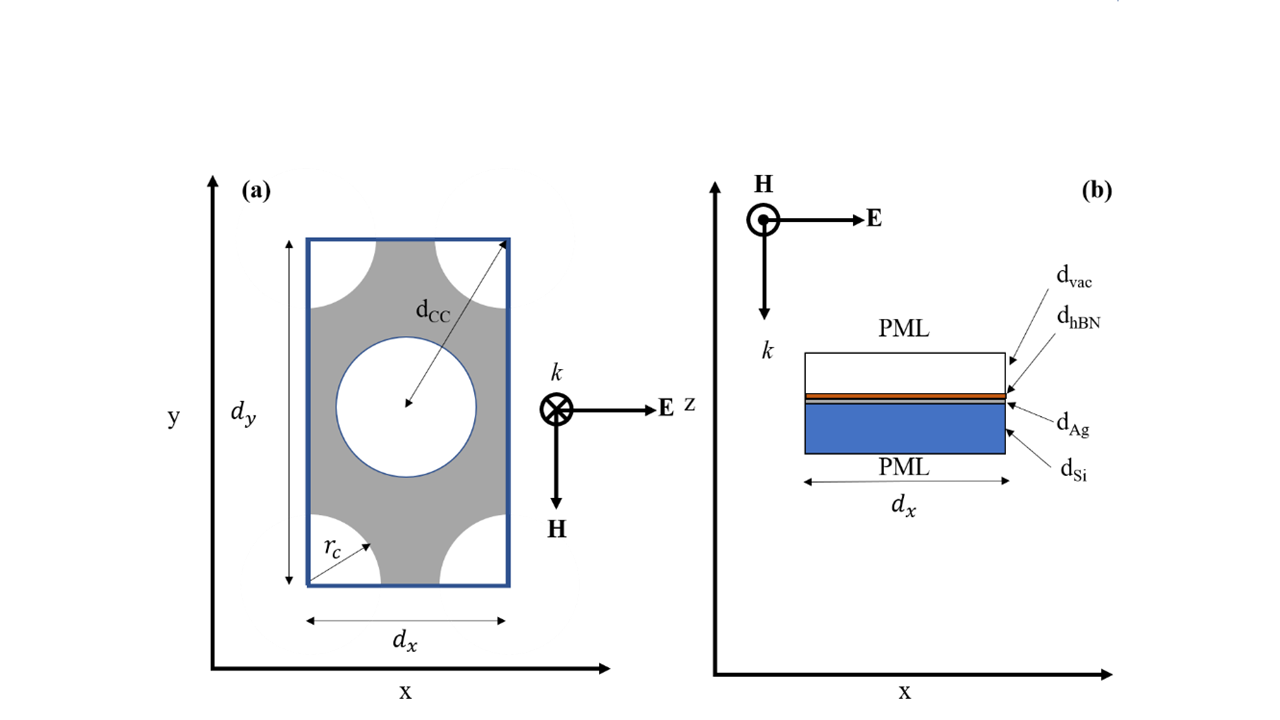
\includegraphics[width=0.9\textwidth]{FiguresCh4/StructurehBNAgHex.png}
        \caption{Schematic of the hBN/Ag structure simulated on this work. \textbf{(a)} Plane view at the hBN/Ag interface. The symmetry reduced unit cell is outlined in red. \textbf{(b)} Cross-sectional view. CPML: Convolutional perfectly matched layer boundary conditions terminated the z direction boundaries. Periodic boundary conditions terminated the x and y boundaries. The unit cell lengths in the x- and y- directions are $d_{x} $ and $d_{y}$, respectively. The layer thicknesses beyond the CPMLs were $d_{\rm{VAC}} = 0.87$ $\rm \mu$m, $d_{\rm{hBN}} = 80$ nm, $d_{\rm{Si}} = 1.0$ $\rm \mu$m, $d_{\rm{Ag}} = 50$ nm. The radius of the holes is $r_{C} = 0.68$ $\rm \mu$m. The distance between the centers of the cylindrical holes is $d_{CC} = d_{x} $. The directions of the \textbf{\textit{E}}-field, \textbf{\textit{H}}-Field and propagation vector \textbf{\textit{k}} is shown in both panes.}
        \label{fig:1}
      \end{figure*}

    The details of the nanopatterned structure simulated in this work are shown in Figure ~\ref{fig:1}. The structure comprised of an 80 nm sheet of hexagonal boron nitride (hBN) deposited on a 50 nm thick film of nanopatterned Ag atop of a Si substrate. The Ag film was patterned with circular holes of radius 0.68 $\rm \mu m$ arranged in a hexagonal lattice with a distance between the centers of $\rm d_{CC}$, which was varied during this work.
\bibliography{hBNPaper.bib}
\end{document}		